\chapter{Essential Files - Input}
Each simulation requires the presence of five files which hold the various input data. Those files are required to have the same base (with the exception of the .tremolo file, see there) name, which we call the project name and are distinguished by a particular suffix. The files are:
\begin{itemize}
 \item \texttt{\$PROJECTNAME.tremolo} (\ref{.tremolo})
\item \texttt{\$PROJECTNAME.potentials} (\ref{.potentials})
\item \texttt{\$PROJECTNAME.validates} (\ref{.validates})
\item \texttt{\$PROJECTNAME.data} (\ref{.data})
\item \texttt{\$PROJECTNAME.parameters} (\ref{.parameters})
\end{itemize}
In the following subsections we describe the options to be set within each file in detail. As a general rule, comments can be added to each file, by starting a line with the \#-Symbol and may be placed almost anywhere. The same is true for empty lines. Most options can also be placed in any order, however there are some, where order is relevant, since they influence each other and even less, which require a specific order simply for the parser to function properly. Those exceptions are mentioned at the descriptions below.

Additionally there are two optional files, \texttt{\$PROJECTNAME.external} and \texttt{\$PROJECTNAME.exttypes}

\paragraph{Working with the GUI\\}
When using the GUI the five mandatory files are automatically generated when creating a new project (which can be done via the drop-down menu or the corresponding ``empty sheet'' icon.
When loading an existing project, all files must be present though, otherwise the project cannot be properly loaded. For the layout of the main options see figure \ref{GUIoptions}.
\begin{figure}
\centering
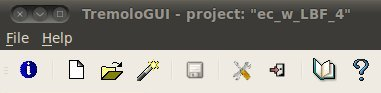
\includegraphics{visuals/GUI_Options.jpg}
\caption{The menu bar in the Tremolo-X GUI. Buttons from left to right:
Project information, new project, open project, creation wizard (not implemented), save project, GUI settings and preferences, GUI exit, GUI help}
\label{GUIoptions}
\end{figure}

\section{\$PROJECTNAME.tremolo} 
\label{.tremolo}
This file could in theory also be named \$ANYTHING.tremolo, with anything deviating from the projectname designated in the file.

\begin{lstlisting}
 global: defaultpath="./$BASENAME";
\end{lstlisting}
The default path is used to allow the use of project independent input files. When the program does not find a specific input file in the current directory, it checks the defaultpath for that file. Since the file may have a basename different from the current project, the basename needs to be specified at all times.

\begin{lstlisting}
global: projectname="$PROJECTNAME";
\end{lstlisting}


Here you actually specify the prefix of all other input files present, which will also be the prefix of the generated output files.
\begin{lstlisting}
global: systemofunits=$SYSTEM_OF_UNITS; 
\end{lstlisting}
This parameter is quite essential as you can choose or customize the system of physical units you wish to use in a particular simulation. The choice made here affects almost any numeric parameter in the simulation and numeric values in other parameter files are expressed in units of the system chosen here.
The options are:
\begin{lstlisting}
 kcalpermole, evolt, si, custom
\end{lstlisting}

\begin{center}
    \begin{tabular}{*{4}{c}}
        \toprule
        {} & kcalpermole & evolt & si \\
        \midrule
        length      & \SI{1}{\angstrom}         & \SI{1}{\angstrom}         & \SI{1}{\meter} \\
        time        & \SI{4.88719e-14}{\second} & \SI{1.01805e-14}{\second} & \SI{1}{\second} \\
        mass        & \SI{1}{\atomicmass}       & \SI{1}{\atomicmass}       & \SI{1}{\kilogram} \\
        current     & \SI{3.27832e-6}{\ampere}  & \SI{1.57377e-5}{\ampere}  & \SI{1}{\ampere} \\
        temperature & \SI{503.556}{\kelvin}     & \SI{11604}{\kelvin}       & \SI{7.2429638e+22}{\kelvin} \\
        \bottomrule
    \end{tabular}
\end{center}
\todo{Check whether the current-unit in kcalpermole is ampere.}

Note, that there is a relation between the scale of the temperature and the energy, which is derived from length, time and mass units. This must be computed individually by the user by dividing the energy by the boltzmann constant.
Below we provide a sample calculation for the eV scaling:
\begin{lstlisting}
# x     sigma = 1 angstrom = 1.e-10 m
# E     u* (sigma/alpha)^2 = epsilon = 1 eV = 1.6021765e-19 kg m^2 / s^2
# t     alpha = 1.0180505e-14 s
# m     u = 1.6605387e-27 kg
# T     epsilon / k_b = 11604.506 K
\end{lstlisting}


\bigbreak

If the choice \texttt{custom} is selected, units must be specified separately according to the following scheme:

\begin{lstlisting}
custom: lengthunit               = {angstrom, nm, m};
custom: lengthscalingfactor      = 1.0;
custom: timeunit                 = {fs, ps, s};
custom: timescalingfactor        = 1.0;
custom: massunit                 = {u, kg};
custom: massscalingfactor        = 1.0;
custom: currentunit              = {"e/s", A};
custom: currentscalingfactor     = 1.0;
custom: temperatureunit          = {K};
custom: temperaturescalingfactor = 1.0;
\end{lstlisting}

By setting any of \texttt{\$PHYSICAL\_QUANTITYscalingfactor} to a value different than $1.0$ all derived physical quantities are affected as well. Thus when using generated output values you need to remember to extract any scaling you introduced here. (Whether you need to divide or multiply, either the factor alone or its square depends on the specific quantity and its units.)


\subsection{Optional input}
\begin{lstlisting}
global: comment="Some comment";
\end{lstlisting}
The comment will be printed to the standard output when the simulation is run.

\subsection{Working with the GUI}
In the GUI this file is controlled by the creation dialog and the first tab. In the creation dialog default path and \$PROJECTNAME must be specified.
\begin{figure}
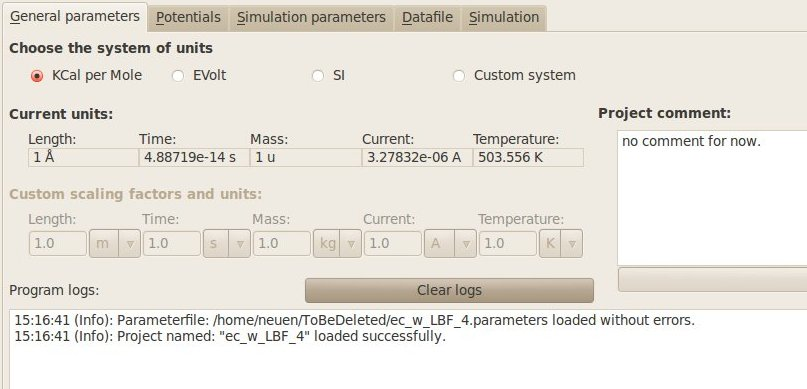
\includegraphics[width=13cm]{visuals/GUI_Main2.jpg}
\caption{}
\end{figure}

\section{\$PROJECTNAME.potentials}
\label{.potentials}
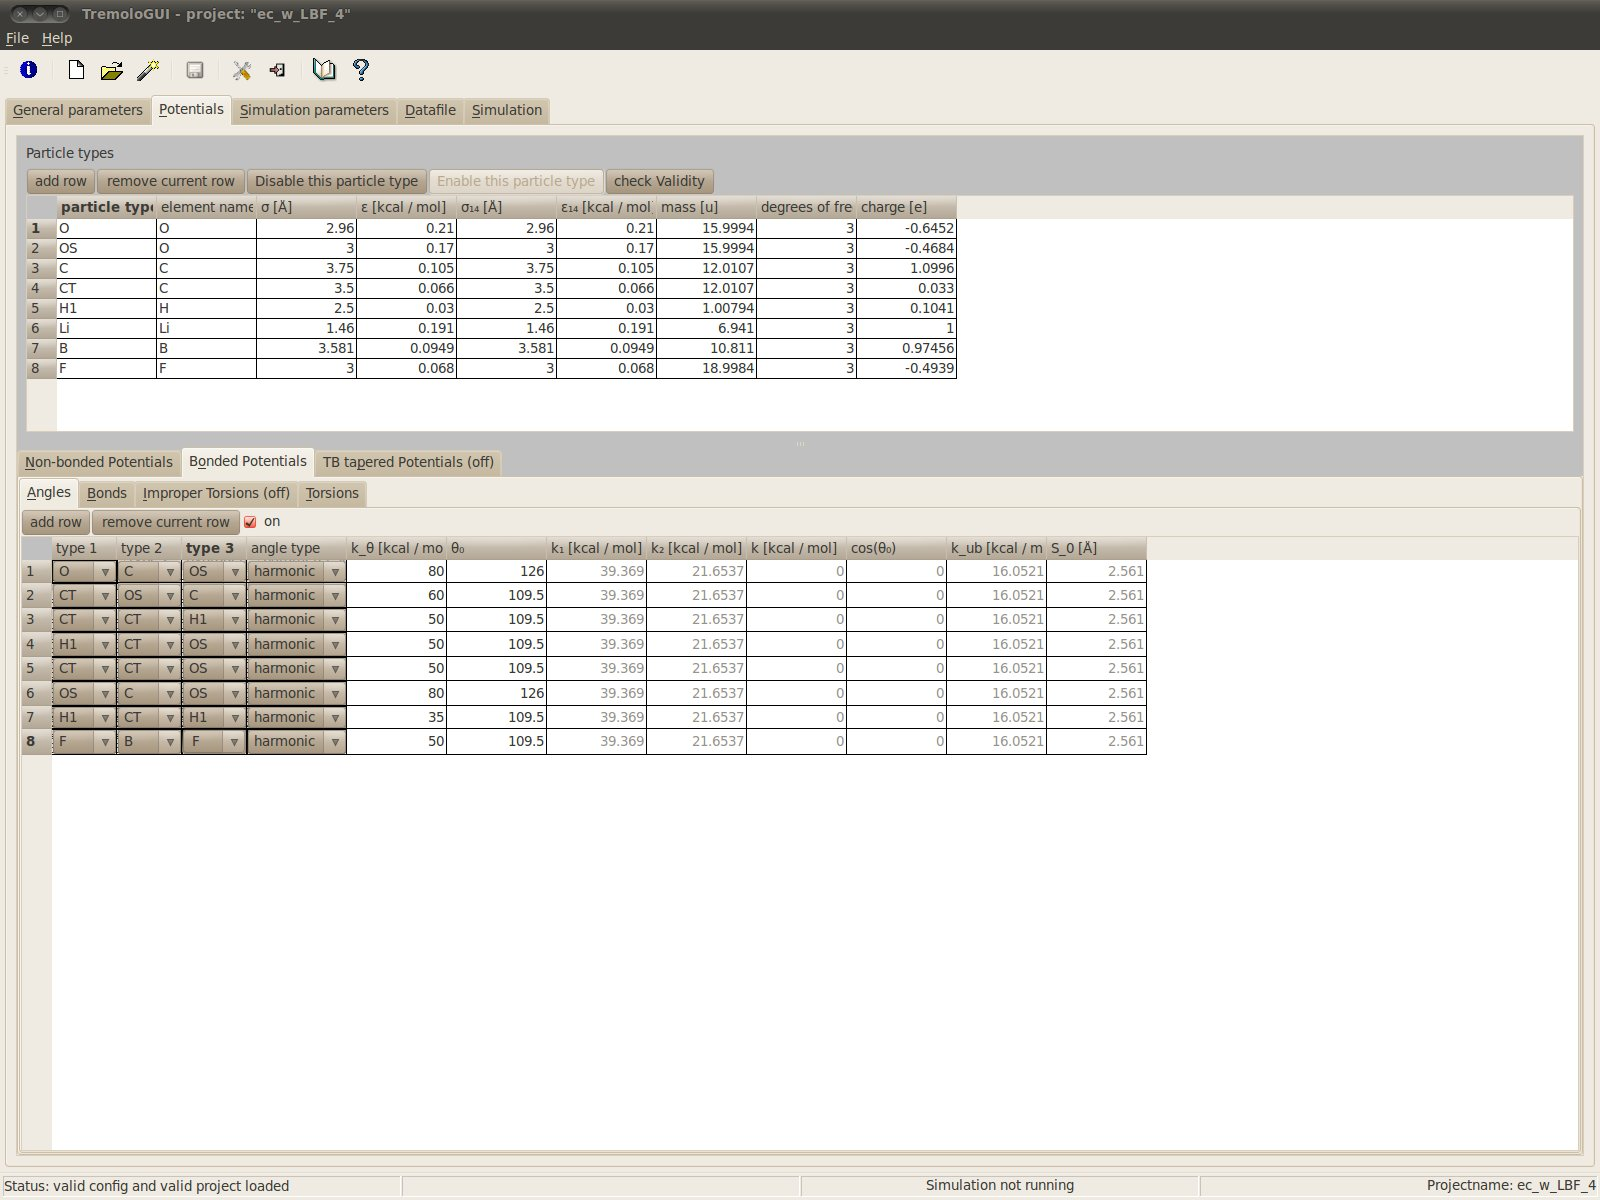
\includegraphics[width=15cm]{visuals/GUI_Potentials_Bonded.jpg}
The potentials file is responsible for all parameters, which affect the forces between atoms in the simulation. It begins with a list of all particle types present in the ensemble, together with some particles which are used more than once: \todo{layout}
{\small
\begin{lstlisting}
 particles	{
 particle: particle_type=$P1, element_name=$NAME1, sigma=1, epsilon=1, sigma14=1, epsilon14=1,    mass=1,    free=3, charge=0;
 particle: particle_type=$P2, element_name=$NAME1, sigma=3, epsilon=1, sigma14=3, epsilon14=0.17, mass=15.9, free=3, charge=-0.4684;
};
\end{lstlisting}
}
The file then lists the potentials, grouped by the type of potential. Each particle requires a specific set of parameters, which, again depending on the type of potential, need to be listed for all pair types (tripled types, ...) of particles to which it shall apply.\todo{layout}
\begin{lstlisting}
nonbonded_2body_potentials      {
   lennardjones:  particle_type1=$P1,  particle_type2=$P1,  r_cut=12.5;
   lennardjones:  particle_type1=$P1,  particle_type2=$P2,  r_cut=12.5;
   lennardjones:  particle_type1=$P2,  particle_type2=$P2,  r_cut=12.5;
   ljspline:      particle_type1=$P1,  particle_type2=$P1,  r_cut=12.5,  r_l=11;
   ljspline:      particle_type1=$P1,  particle_type2=$P2,  r_cut=12.5,  r_l=11;
   ljspline:      particle_type1=$P2,  particle_type2=$P2,  r_cut=12.5,  r_l=11;
        };
\end{lstlisting}

\todo{Make entry for each potential.}

\section{\$PROJECTNAME.validates}
\label{.validates}

All particles and force fields detailed in the .potentials file need to be validated in this file, by setting their state to on. The reason for this is the converse action, this allows to selectively deactivate particle types and force fields, which shall not be used in this particular situation. This might be relevant, if you wish to experiment with several different (combinations of) force fields: Instead of writing an entire .potentials file for each combination, one such file with all desired forcefields is sufficient and you only need to make minor changes to the .validates file.

\begin{lstlisting}
validate: particle_type=$P1, state=on;
validate: particle_type=$P2, state=off;

validate: force_type=lennardjones, state=off;
validate: force_type=ljspline, state=on;
\end{lstlisting}


\section{\$PROJECTNAME.data}
\label{.data}
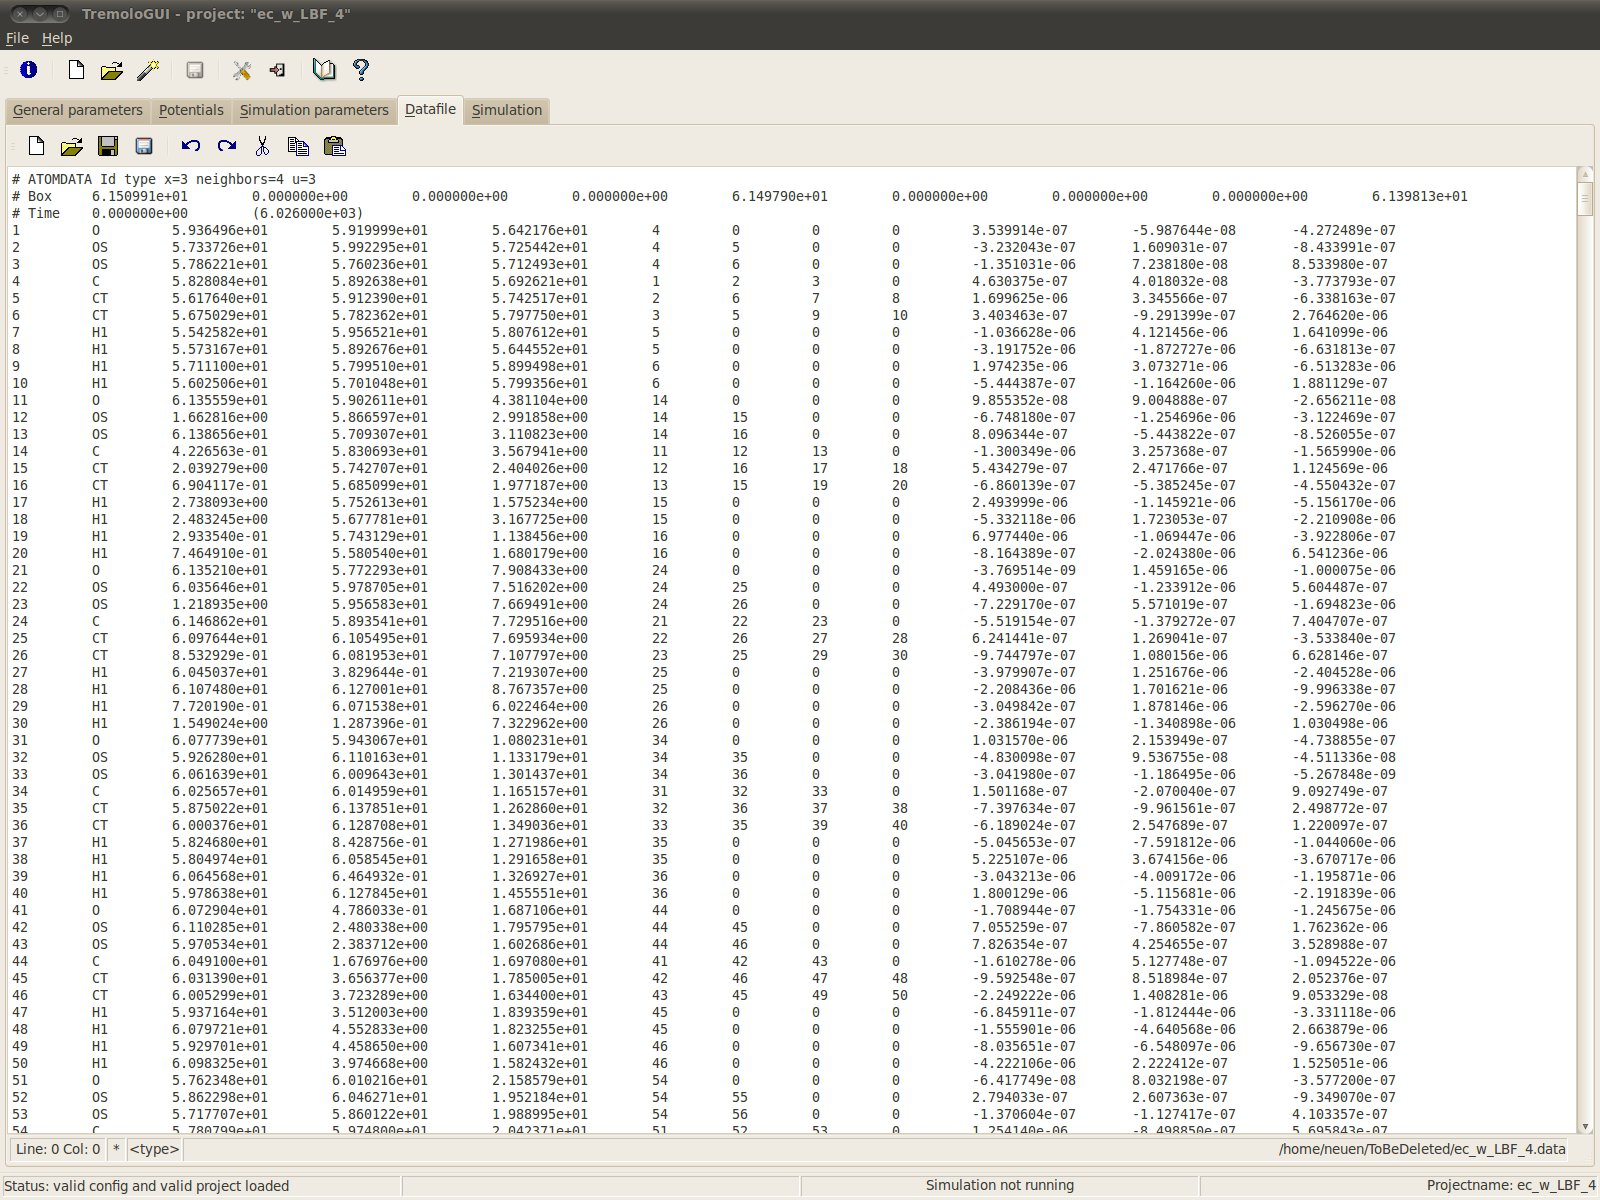
\includegraphics[width=15cm]{visuals/GUI_Data.jpg}

This file contains all information about the initial configuration of the atoms. Always present is the line \texttt{ATOMDATA} line, which informs the parser about the type and order of the input. It may be followed by some optional \texttt{ATOMDATAADDOUT}, \texttt{INPUTCONV} and \texttt{OUTPUTCONV} lines.
\begin{lstlisting}
ATOMDATA  <record_entry_1> ... <record_entry_n>
 <record_entry>: <dataname>[=<n>]
 <dataname>    : x | xs | u | F | stress | Id | charge | GroupMeasureTypeNo | type | neighbors | extType | imprData | name | resName | chainID | resSeq | occupancy | tempFactor | segID | Charge
               
\end{lstlisting}



In the example below the line specifies the options \texttt{Id} and \texttt{type}, which occupy a single column each. This is followed by the particle positions \texttt{x}, which require a three column wide vector, neighbors with a four column vector and finally velocities \texttt{u}, which use three columns again. Note that all options are case sensitive.\todo{layout}
{\tiny
\begin{lstlisting}
# ATOMDATA Id type x=3 neighbors=4 u=3
1       O       5.936075e+01    5.915340e+01    5.643238e+01    4       0       0       0       3.540887e-07    -5.986875e-08   -4.272449e-07   
2       OS      5.734245e+01    5.991388e+01    5.725724e+01    4       5       0       0       -3.232931e-07   1.608824e-07    -8.433911e-07   
3       OS      5.782428e+01    5.758512e+01    5.712316e+01    4       6       0       0       -1.351403e-06   7.237250e-08    8.533900e-07    
4       C       5.826889e+01    5.890171e+01    5.693151e+01    1       2       3       0       4.631648e-07    4.017515e-08    -3.773758e-07  
\end{lstlisting}
}
Possible options and their meaning are:
\begin{itemize}
\item \texttt{type} (string) This parameter must be present and it must match one of the particle types specified in the .potentials file.

\item \texttt{Id} An identifier for each particle. When this parameter is used id numbers need to be assigned sequentially, 
  otherwise there may be unexpected behavior. This is a requirement for the use of \texttt{neighbors}.

\item {\tt x=3} This are the carrtesian coordinates. The only sensible vector length is three.

\item {\tt xs=3} This are the scaled/fractional coordinates. The only sensible vector length is three. Note that {\tt x=3} or {\tt xs=3} must be given.

\item {\tt u=3} If one wishes to give particular velocities to individual particles, this can be specified here. In the case of a dynamics simulation it is set by default for the data output files. This way, you are able to restart the simulation from the finishing point. 
  Supplying starting velocities also fixes an initial temperature and may conflict with the corresponding option 
  \ref{INPUTCONV}, which takes precedence. The only sensible vector length is three.

\item {\tt neighbors=<n>} This parameter(-vector) specifies the particles to which the present one is bonded by specifying 
  its {\tt Id} number. The identifier {\tt Id} numbers must exist and a particle may not be linked to itself. For non-bonds, 
  enter a zero instead. The length of this vector can be any positive integer. This is relevant for bonded force fields.

\item {\tt charge} This parameter fixes an (electric) charge for this parameter. To have an effect, some Coulomb 
  potential must be used. (This overwrites the charge set in the .potentials file for the particle type \todo{test whether this is correct.}

\item {\tt F=3} This option allows to write out the current forces on each particle at the output time step.
  \todo{It is advised to start with zero entries in these columns. The necessity should be verified.}

\item {\tt stress=<n>} This allows the output of this particles contribution to the total box stress. 
  While not a physical stress value by itself (point particles do not have stress) this allows to determine 
  local stress in a macro-structure by comparison among the particles. In the case you set the option in the parameter file to measure the local stress, it is set by default for the data output files.

\item {\tt imprData=<n>} When using improper torsion forces, use this as {\tt neighbors} in order to specify 
  neighbors for the respective force.

\item {\tt GrpTypeNo} For certain measurement routines, particles may be assigned to groups, which do not need 
  to respect particle types. \todo{specify relevant options, 4 indices?}
\end{itemize}
The information below belongs to PDB information, they are only parsed in and written out, they have no effect on simulation
\begin{itemize}
\item {\tt extType} type number used for external forces \todo{Is this actually a PDB option?}
\item {\tt name} particle name (used only for PDB data)
\item {\tt resName} residue name (used only for PDB data)
\item {\tt chainID} chain ID (used only for PDB data)
\item {\tt resSeq} residues sequence number (used only for PDB data)
\item {\tt occupancy} occupancy (used only for PDB data)
\item {\tt tempFactor} temperature factor (used only for PDB data)
\item {\tt segID} segment ID (used only for PDB data)
\item {\tt Charge} Charge (string) (used only for PDB data)
\end{itemize}
For the proper handling of PDB parameters, this feature must have been enabled at configure time of Tremolo-X. \todo{Discuss enable by default.}

You can use an ATOMDATAADDOUT line in the same way to output additional data in the data output files, e.g. to write out forces in the above example:
 \begin{lstlisting}
# ATOMDATA Id type x=3 neighbors=4 u=3
# ATOMDATAADDOUT F=3
\end{lstlisting}

Note that one can also give the box matrix by a \texttt{\# BOX} line
in the \texttt{.data} file. In particular, a \texttt{\# BOX} line
given in the \texttt{.data} file will overwrite values from the
\texttt{.parameter} file.
\begin{lstlisting}
# BOX xx xy xz yx yy yz zx zy zz
\end{lstlisting}

\subsection{Input conversion}
\label{INPUTCONV}
The .data file may contain options, which influence the starting configuration of the sample. In the following list, {\tt \{0|1\} } indicates that the option is activated by setting the integer to 1, while it is deactivated with 0. The default behavior (on/off) depends on the option and is listed.
\begin{itemize}

\item {\tt \# INPUTCONV shift} Shift of initial particle coordinates by specifying a vector or by positioning the {\tt (0. 0. 0.)} 
  coordinate in the center of the simulation domain (this would be equivalent to the half of the diagonal vector of the simulation domain.) 
  Either supply vector {\tt x y z} or write {\tt center}. Note that the shift vector is given in scaled/fractional coordinates, e.g.\ the center is  {\tt (0.5 0.5 0.5)}.
\item {\tt \# INPUTCONV trans} Transformation of initial particle coordinates by a matrix {\tt A} (which needs to be supplied as: 
  {\tt <A\_xx> <A\_xy> <A\_xz>  <A\_yx> <A\_yy> <A\_yz>  <A\_zx> <A\_zy> <A\_zz>}) Transformation is done after shifting. Note that the transformation is applied on scaled/fractional coordinates.
\item {\tt \# INPUTCONV periodic 1|0} Enable/Disable periodic correction for coordinates of inserted particles.
  This feature is active by default.
\item {\tt \# INPUTCONV temp \#FLOAT} is specified all particles are assigned a Maxwell-Boltzmann distributed velocity, 
  such that the total kinetic energy corresponds to the temperature value specified (in units of the chosen system. 
  Using this option overwrites any user specified velocities. Note that the kinetic energy will most likely change over 
  the course of the simulation, unless a thermostat is in use.
\item {\tt \# INPUTCONV moment 0|1} results in the computation of the total momentum and a correction of all particle velocities,
  such that the new momentum is zero at the start of the simulation. Note that the use of a thermostat, 
  while maintaining the kinetic energy might cause the momentum to change over the course of the simulation runtime. 
  (On the momentum conservation of thermostats, see section \ref{thermostats}) This feature is inactive by default.
\item {\tt \# INPUTCONV angmoment 0|1} results in the computation of the total angular momentum and a correction of all particle velocities, 
  such that the new angular momentum is zero at the start of the simulation. Note that the use of a thermostat, 
  while maintaining the kinetic energy might (will most likely) cause the angular momentum to change over the course of the simulation runtime. This feature is inactive by default.
\end{itemize}
Note that \# is always part of the command. Thus, comments may not be added to this file, as they would interfere with the parsing of the regular commands.


If both momentum correction and temperature distribution are set, then first the
temperature distribution is set, then the moment is corrected, then the velocities
are scaled again to match the temperature.

 Example file:
\# ATOMDATA x=3 type
\# INPUTCONV shift center
\# INPUTCONV temp 0.57
\# INPUTCONV moment 1
\# INPUTCONV angmoment 1
0 0 0 C
0 1 0 H
0 0 1 H
\subsection{Output conversion}
\label{OUTPUTCONV}


\section{\$PROJECTNAME.parameters}
\label{.parameters}

This file contains the most extensive set of options, which may also interfere with each other. Therefore, this section only serves to explain the syntax of the file, while the comprehensive explanation of the option is moved to the following chapters.

The basic syntax scheme is the following:
\begin{lstlisting}
$ITEM1: $PARAMETER1=#VALUE, $PARAMETER2=#values;
$ITEM2: $PARAMETER1=#VALUE;
$CATEGORY {
       $ITEM1: $PARAMETER1=#VALUE;
       $ITEM2: $PARAMETER1=#VALUE, $PARAMETER2=#values, ... ;
       $SUBCATEGORY  {
                $ITEM1: $PARAMETER1=#VALUE;
                $ITEM2: $PARAMETER1=#VALUE, $PARAMETER2=#values, ... ;
                $ITEM3: $PARAMETER1=#VALUE, $PARAMETER2=#values;
                  };
            };
};
\end{lstlisting}
Modifications from this scheme occur for the propagator and timelines\fixme{Timelines working?} and are described there in detail.



With two exceptions the parameters are grouped into the following categories:
\begin{itemize}
 \item domain \ref{sub:domain}, \ref{domain}
 \item optimization \ref{sub:optimization}, \ref{optimization}
 \item dynamics \ref{sub:dynamics}, \ref{ensembles}
 \item coulomb \ref{sub:coulomb}, \ref{longrange}
 \item parallelization \ref{sub:parallelization}, \ref{parallelization}
 \item output \ref{sub:output}, \ref{measurement}
\end{itemize}

There are two parameters, which are not associated with any of the above categories. The basic choice, whether the simulation type should be optimization or dynamics, determines, whether the parser takes options from the dynamics section or from the optimization section:
\begin{lstlisting}
 integration: type=$TYPE;
\end{lstlisting}
where \$TYPE = \{\textit{dynamics, optimization}\}.
\bigbreak
The other stand alone parameter is the cut``radius'' of the linked cells, which is set by
\begin{lstlisting}
 lcs:    cellrcut=#FLOAT;
\end{lstlisting}
where \#FLOAT is a positive floating point number. Also, the \texttt{cellrcut} must be smaller than the box dimensions or in case of parallel computations smaller than the box length divided by the number of processes in each direction.

Example: Your domain is 15x15x16. If you employ 3x3x3 processes, your \texttt{cellrcut} may not exceed 5. If you employ 3x3x4 processes your \texttt{cellrcut} may not exceed 4.

It is sensible to choose the \texttt{cellrcut} just as small, that cut off radii of pair potentials just fit into one cell~\cite{GriebelEng}.

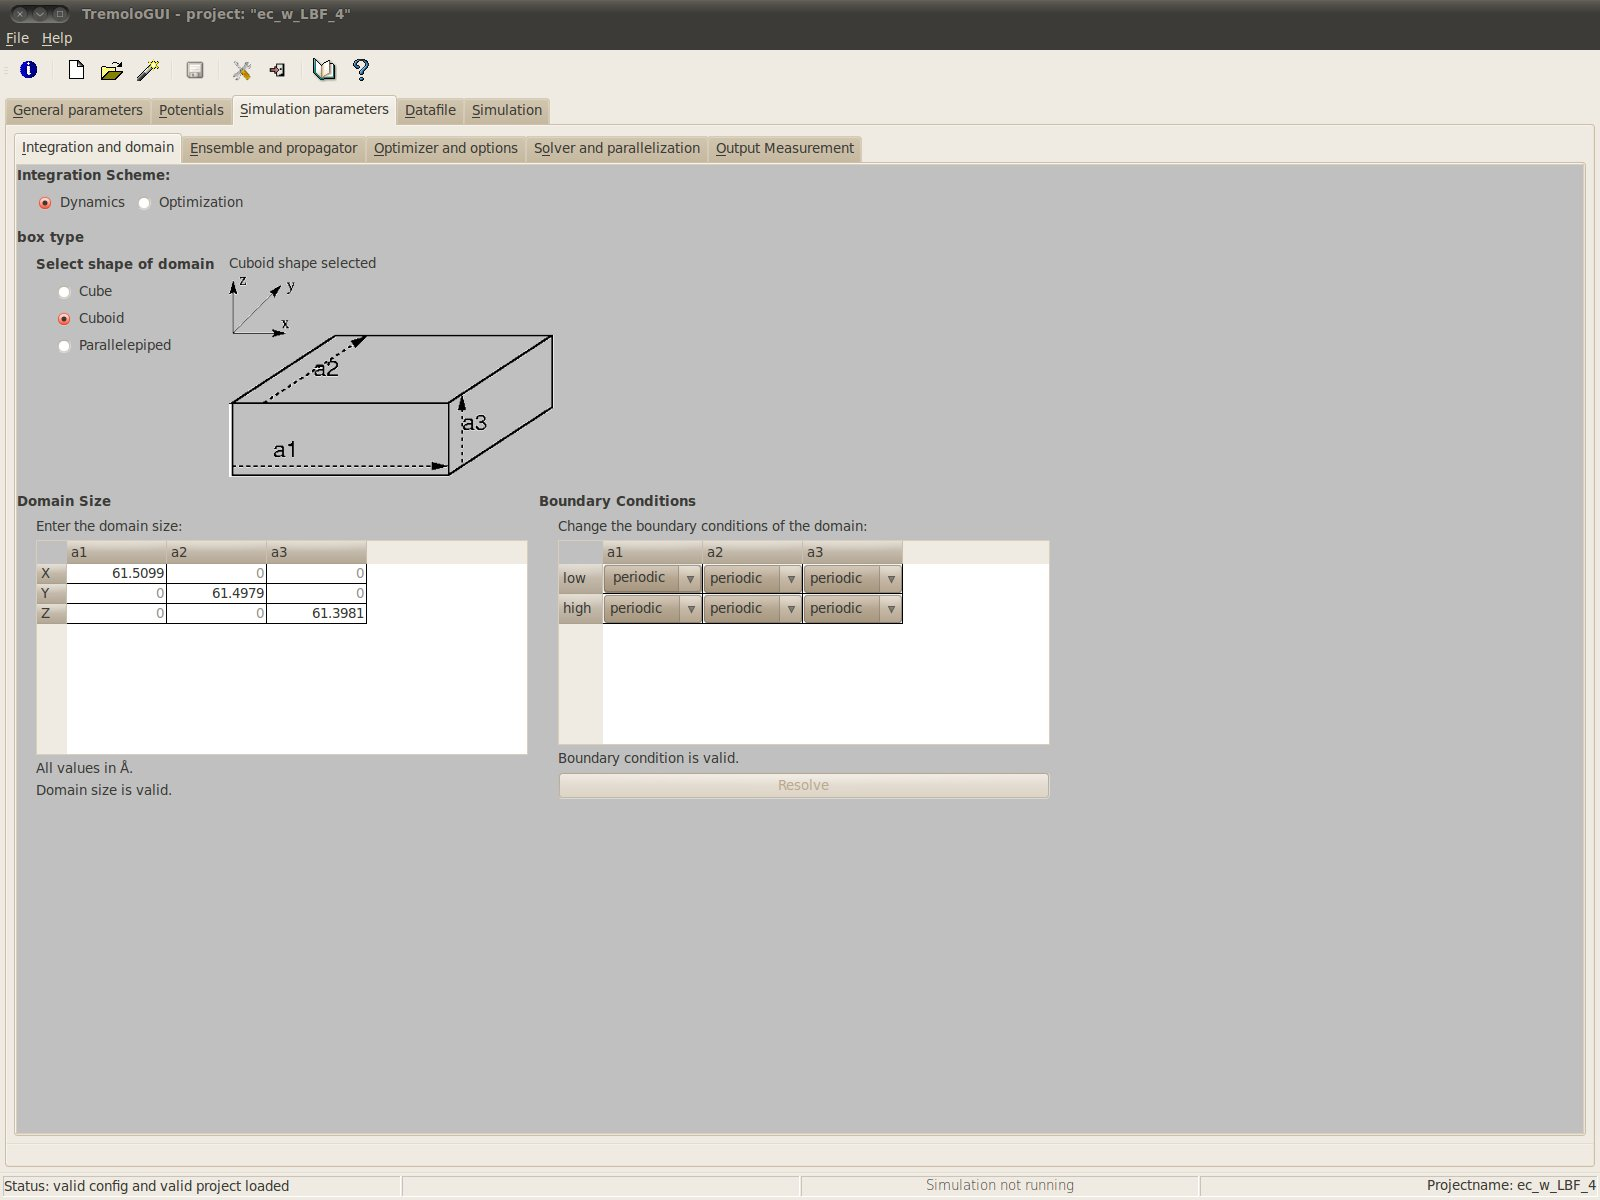
\includegraphics[width=15cm]{visuals/GUI_Parameter_Integration_Domain.jpg}
\subsection{domain}
\label{sub:domain}

The category domain contains the items:
\begin{lstlisting}
size:
type     = {cube, diag, matrix},
size     = #FLOAT,
length_x = #FLOAT, length_y = #FLOAT, length_z = #FLOAT,
xx = #FLOAT, xy = #FLOAT, xz = #FLOAT,
yx = #FLOAT, yy = #FLOAT, yz = #FLOAT,
yx = #FLOAT, zy = #FLOAT, zz = #FLOAT;
\end{lstlisting}

Depending on the type specified, you may leave out the size entries for the other categories, e.g. 
\begin{itemize}
 \item for {\tt cube} you only need to specify \texttt{size}, which is a uniform edge length,
 \item for {\tt diag} you need to set \texttt{length\_x, length\_y and length\_z},
 \item for matrix you need to set the edge vector in the matrix (There are vectors x,y,z with components x, y, z.).
\end{itemize}
The other specifiers may be omitted, however if you supply them the programm will ignore them safely.

Note that one can also give the box matrix by a \texttt{\# BOX} line
in the \texttt{.data} file. In particular, a \texttt{\# BOX} line
given in the \texttt{.data} file will overwrite values from the
\texttt{.parameter} file.
\begin{lstlisting}
# BOX xx xy xz yx yy yz zx zy zz
\end{lstlisting}

\begin{lstlisting}
border:
bt_xlow  = {periodic, leaving, reflecting},
bt_xhigh = {periodic, leaving, reflecting},
bt_ylow  = {periodic, leaving, reflecting},
bt_yhigh = {periodic, leaving, reflecting},
bt_zlow  = {periodic, leaving, reflecting},
bt_zhigh = {periodic, leaving, reflecting};
\end{lstlisting}

The options {\tt leaving} and {\tt reflecting} may be mixed, whereas {\tt periodic} must always match for the respective low and high borders.

\subsection{dynamics}
\label{sub:dynamics}
we have the items:
\begin{lstlisting}
ensemble:       ensemble={NVE, NVT, NPT, NPE};
\end{lstlisting}
\begin{lstlisting}
propagator,     $INTEGRATOR: delta_T=#FLOAT,  endtime=#FLOAT,     timeinteps=#FLOAT,       maxiteration=#INTEGER;
\end{lstlisting}
%$

\$INTEGRATOR = \{{\tt verlet, beeman2, beeman3, beeman4, beeman5, beeman2v, beeman3v}\}

The parameters \texttt{timeinteps} and \texttt{maxiteration} are only relevant in the case of an velocity type algorithm, they are used for aborting the iteration procedure, either when the iterative error drops below \texttt{timeinteps} or the number of iteration cycles reaches \texttt{maxiteration}.

\subsubsection{thermostat}
The subcategory \textbf{thermostat}
%\begin{lstlisting}nose:   	    state={on, off},      F_Mass=#FLOAT;\end{lstlisting}
\begin{lstlisting} nosehoover:         state={on, off},      F_Mass=#FLOAT; 
\end{lstlisting}
\begin{lstlisting}
berendsen:          state={on, off},      T_Interval=#FLOAT;
\end{lstlisting}
%\begin{lstlisting}dpd:    	    state={on, off},      gamma=#FLOAT,        r\cut=#FLOAT;\end{lstlisting}
\begin{lstlisting} constanttargettemp: state={on, off},      T_Temp=#FLOAT;
\end{lstlisting}
%\begin{lstlisting}timeline:          state={on, off},      [time,  temperature,    interpolation=(0,     0,      constant)];\end{lstlisting}
\todo{nose, dpd, timeline (working?)}

\subsubsection{barostat}                   
The subcategory \textbf{barostat}
{\small
\begin{lstlisting}
parinello: state={on, off},      f_mass=#FLOAT;
constraint: type={isotropic, standard, symmetric, none};
constraintmap: xx={0|1}, xy={0|1}, xz={0|1}, yx={0|1}, yy={0|1}, yz={0|1}, zx={0|1}, zy={0|1}, zz={0|1};
constantpressure: state={on, off},       Pressure=#FLOAT;
Timeline: state={on, off},      [time,  pressure,  interpolation=(0, 0, constant)];
stresstensor: [time,  stress, interpolation, xx, xy, xz, yy, yz,zz=(0, 0, constant, 0, 0, 0, 0, 0, 0)];
\end{lstlisting}
}

For theoretical background and detailed description of the options see section \ref{section:ensembles:barostat}.
The first option obviously switches the barostat on/off. The second option determines the virtual mass
assigned to the box.
In the constraint line one of the four constraint types must be chosen, which will work together with the 
following selection from the constraintmap.
The selection of the constraintmap must always obey symmetry and in the isotropic case the ``1'' entries
must be restricted to the diagonal. It is possible to 


\todo{constraintmap, stresstensor; timeline(working?)}

When a constraint type is chosen, this places certain restrictions on the constraintmap, however the user still needs to set it accordingly. 
(The constraintmap is not locked, since it allows the user to enforce restrictions to subdimensions.)
The constraintmap must always observe \texttt{xy=yx} etc., even for the non symmetric restrictions.
\begin{itemize}
\item The \texttt{isotropic} constraint allows only changes on the main (diagonal) axis. Furthermore those changes are enforced to be isotropic, meaning the changes are identical in all allowed directions. (e.g. the user may set only \texttt{xx} and \texttt{yy} to 1, prohibiting changing of the box in the z direction.)
\item \texttt{standard} the box deformation is restricted to an upper triangular matrix.
\item \texttt{symmetric} constraints enforce symmetry in the box deformation. 
\item \texttt{none} No additional constraints are placed on the deformation tensor. Note that this is unphysical.
\end{itemize}

In the following lines we can specify the mean pressure applied to the system (both as a constant and as a timeline), as well as a stresstensor, 
which is externally applied, independent of the stress exerted by the particles in the system.

\subsection{optimization}
\label{sub:optimization}
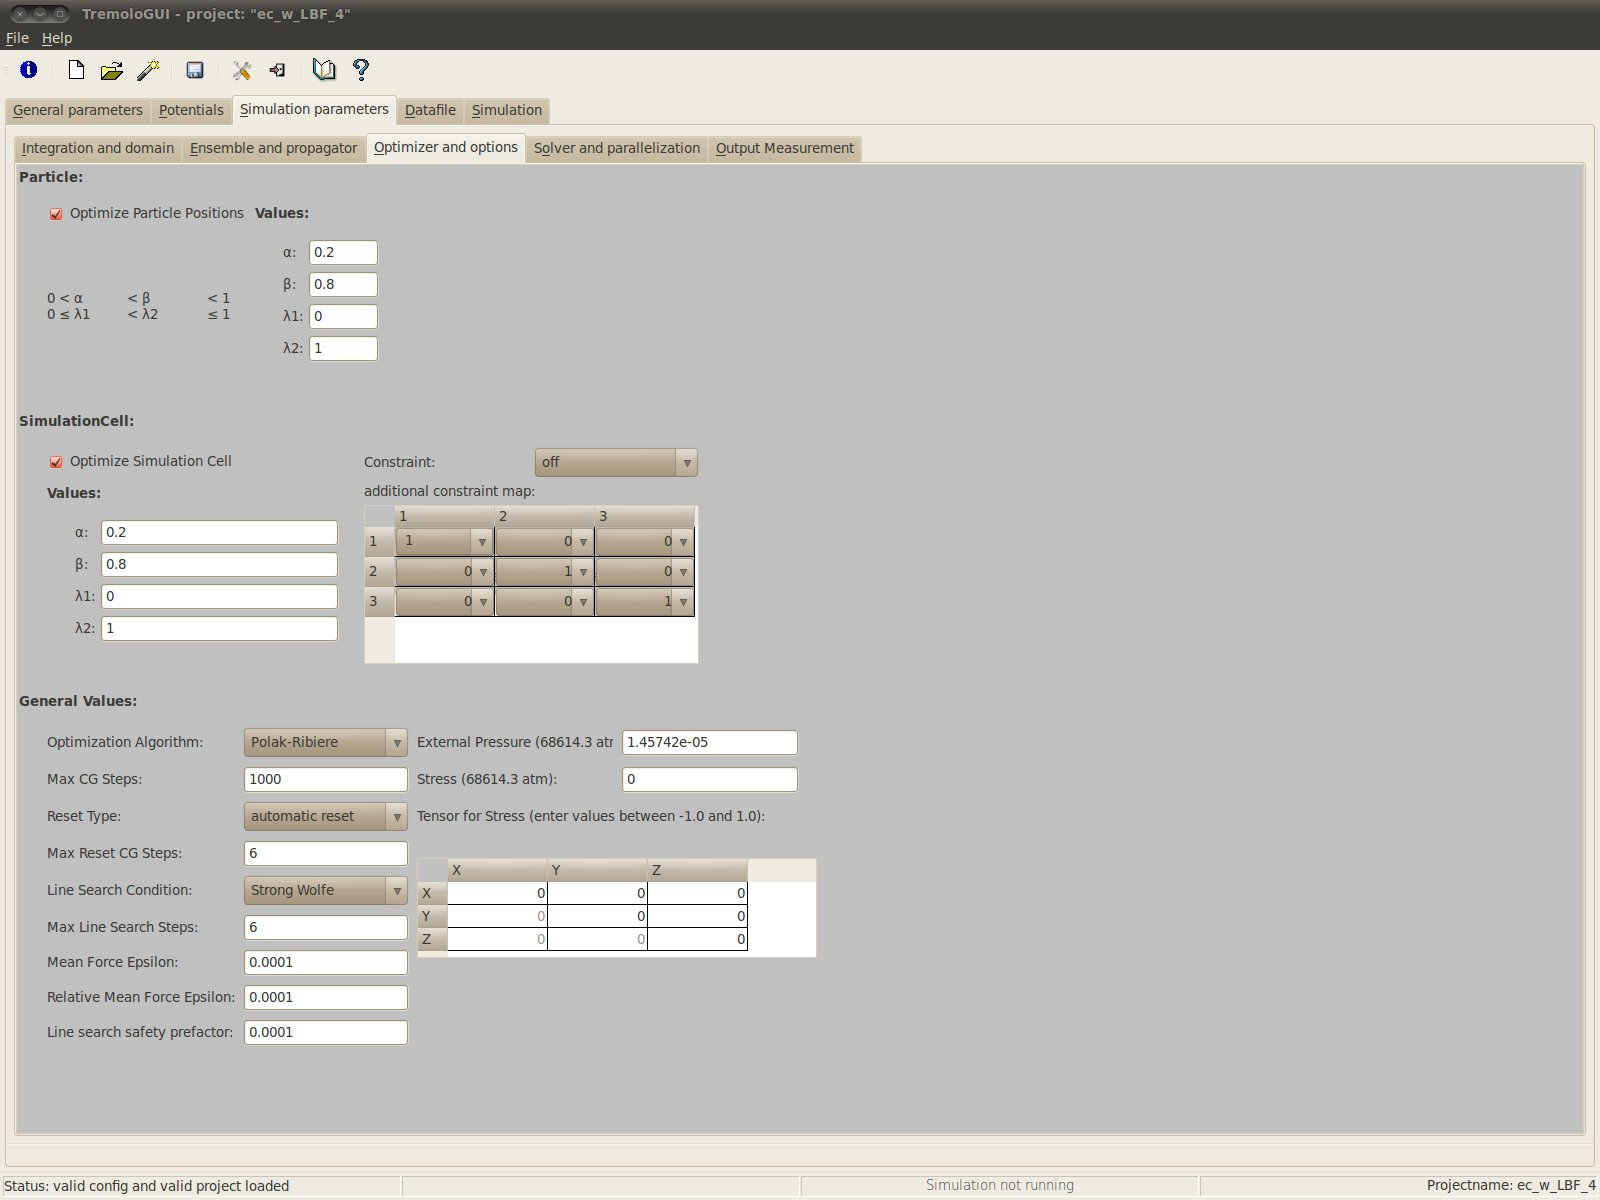
\includegraphics[width=15cm]{visuals/GUI_Parameter_Optimizer.jpg}

\begin{lstlisting}
optimization{
  particle: state=on,  alpha=0.2,   beta=0.8,    lambda1=0,   lambda2=1;
  simucell: state=off, alpha=0.2,   beta=0.8,    lambda1=0,   lambda2=1;
  simucell: constraint=isotropic,  XX=1,  XY=0,  XZ=0,  YX=0,  YY=1,  YZ=0,  ZX=0,  ZY=0,  ZZ=1;
  common:   algorithm=fr,  maxcg=102,  RT=periodical,  maxresetcg=6,  LS=wolfe,   maxlinesearch=6,   mean_force_eps=1e-05,  mean_force_eps_rel=1e-05,  prefactor=0.001, extpressure=1;
  stress:   stress=0,  XX=0,  XY=0,  XZ=0,  YX=0,  YY=0,  YZ=0,  ZX=0,  ZY=0,  ZZ=0;
};
\end{lstlisting}

\todo{complete optimization}
\subsection{coulomb}
\label{sub:coulomb}
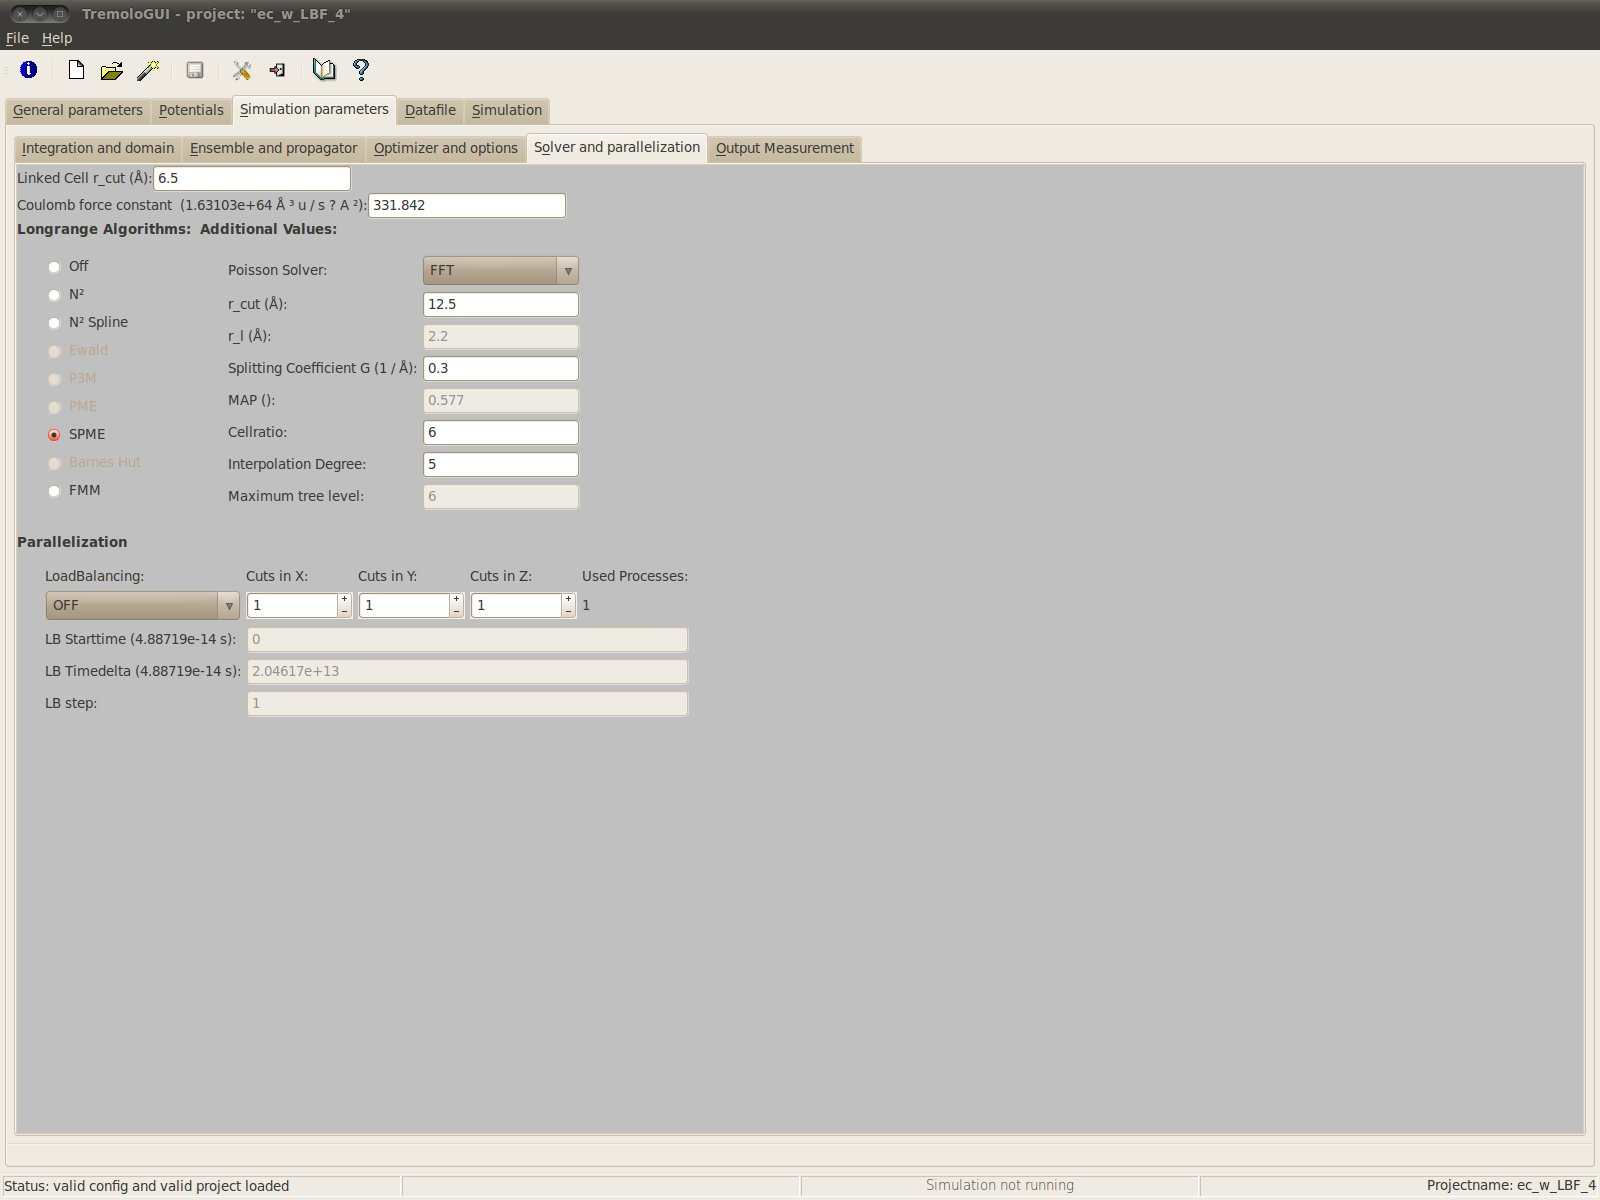
\includegraphics[width=15cm]{visuals/GUI_Parameter_LongRange_Parallel.jpg}
\begin{lstlisting}
coulomb {
permittivity:   epsilon0inv=1.9620959e-21; 
n2:        state=off, r_cut=0.7352941, i_degree=5;
n2spline:  state=off, r_cut=0.7352941, r_l=0.6470588, i_degree=5;
ewald:     state=off, r_cut=0.7352941, G=1.19e-10,    i_degree=5,  cellratio=6;
p3m:       state=off, r_cut=0.7352941, G=1.19e-10,    i_degree=5,  cellratio=6,  ps=fft;
pme:       state=off, r_cut=0.7352941, G=1.19e-10,    i_degree=5,  cellratio=6,  ps=fft;
spme:      state=off, r_cut=0.7352941, G=1.19e-10,    i_degree=5,  cellratio=6,  ps=fft;
barneshut: state=off, r_cut=0.7352941, mtl=6,         i_degree=5;
fmm:       state=off, r_cut=0.7352941, mtl=6,         i_degree=5,  Map=0.577;
};
\end{lstlisting}

Currently \texttt{n2}, \texttt{n2spline} and \texttt{spme} are implemented.

\emph{Note that the \texttt{SPME} method
is not implemented sequentially and requires a Tremolo-X version with parallel capabilities. 
You can start the parallel version with one process though and use SPME nevertheless.}
\subsubsection{Permittivity}
The coulomb-force-constant epsilon0inv is the only constant which is truly associated with units.
(All others are converted to a reduced state.) As such it is dependent on the choice of the unit system. 
In this context it is necessary to note, that there are several different definitions of the calory,
which need to be distinguished.
Despite its name it is not the inverse of $\epsilon_0$.
\begin{equation*}
\text{\tt epsilon0inv}=\frac{1}{4 \pi \epsilon_0} \cdot \frac{e^2}{\left[length\right],}
\end{equation*}
where $e$ is the respective charge unit and $\left[length\right]$ the unit of length used.

A few common examples, which all use the electron charge and angstrom but convert to different reference energies, are:
\begin{itemize} 
\item Using angstrom and kcal$_{th}$/mol:\\
$ \frac{1}{4*\pi*\epsilon_0} * (e^2/angstrom) = 332.06371 \quad kilo cal_{th} / mol N_A$

\item Using angstrom and kcal/mol:\\
$ \frac{1}{4*\pi*\epsilon_0} * (e^2/angstrom) = 331.84164  \quad kcal_{mol}$

\item Using angstrom and eV:\\
$ \frac{1}{4*\pi*\epsilon_0} * (e^2/angstrom) = 14.399644  \quad eV $
\end{itemize}

\subsubsection{r\_cut, r\_l}
The r\_cut parameter determines the separation of short and long range part of the potential. For the case of the splined N$^2$-Algorithm 
r\_l defines the radius from which spline interpolation to the cut-off starts. For more information see section \ref{longrange}.
\subsubsection{i\_degree}
This parameter determines the degree of the polynomials used for the field interpolation.
\subsubsection{G}
Localization parameter for the smooth screening functions. With larger G the localization is tighter.
\todo{Suggest to keep values between 0.24 and 0.35 1/angstrom?}
\subsubsection{cellratio}
Ratio of interpolation nodes per LC cell in one dimension. (Depending on the method this may be enlarged to the next power of two.)
\subsubsection{mtl}
Maximal tree level of the multipole method.

\todo{complete coulomb}


\subsection{parallelization}
\label{sub:parallelization}
Parameters for domain decomposition can be set on the command line when calling the program. If this is done, those parameters supersede and replace those set in the 
{\tt .parameters} file.

\begin{lstlisting}
parallelization {
    proc:     n1=1,   n2=1,   n3=1,   all=1;
    loadbal:  wf=off, Lb\_t=0, Lb\_delta=4.608295e+11,  Lb\_step=1;
};
\end{lstlisting}
\subsubsection{Number of processors}
The numbers {\tt n1}, {\tt n2} and {\tt n3} are the number of cell bins per respective dimension. Their product must equal the total number of processes assigned with {\tt all}.
\subsubsection{Loadbalancing}

\todo{complete parallelization}
\subsection{output}
\label{sub:output}
\begin{lstlisting}
Outvis:  T_Start=0,   T_Delta=10,    Step_Delta=100;
Outm:    T_Start=0,   T_Delta=0.01,  Step_Delta=1;
Outmm:   T_Start=0,   T_Delta=10,    T_Deltam=9,     Step_Delta=10,  Step_Deltam=9;
Outdata: T_Start=0,   T_Delta=5,     Step_Delta=10;
energy:  measure=on,     meanmeasure=off;
analyze  {
         radial:       measure=off,  meanmeasure=off,  vis=off,  r_cut=1.470588,   n_bin=50;
           radialdistribution {
                              radialdist:  particle_type1=CT,  particle_type2=CT;
                              };
         bond:         measure=off,  meanmeasure=off,  vis=off;
           bondDistances {
                         bondDistance:   particle_type1=CT,  particle_type2=CT,  distance=2.700000e+00;
                         };
         velocity:     measure=off, meanmeasure=off,  vis=off,  min=0,  max=0.006382352, n_bin=50;
         msd:          msdusegroups=off;
         msd:          particle_type=Argon, groupno=0, starttime=100, resetinterval=1000, measureflag=1, convection_correction=on/off;
         local_stress: localstress=on/off;
         };
\end{lstlisting}
\subsubsection{Out\{-vis,-m,-mm,-data\}}
See section \ref{measuresetting} for details. Note that measure data is also written, if visual output is created, regardless of the state of the measure output interval. This interval is not touched, so if the intervals do not naturally coincide both are observed. Regardless of whether a measure event has been caused by creation of visual output or expiration of the measure interval, both are written to the same file.

The data stream consists of the current state of particles in terms of the input ({\tt .data}-file). This information is written to {\tt \$PROJECTNAME.data.9999} in the case of serial computation or {\tt \$PROJECTNAME.data.9999.\#\#\#\#} in the parallel case, where {\tt \#\#\#\#} are replaced by a four digit representation of the job number on which the particles where currently placed. (Scripts for merging this are described in \todo{Describe scripts.})
\subsubsection{energy}
Both option take {\tt on} and {\tt off} as arguments. They decide whether measure and/or mean measure are carried out.
\subsubsection{radial}
As a rule, in addition to switching the measurement of the radial distribution on, the user must specify for which pairs of particles the radial distribution shall be computed.
However, the parameters set apply to all pairs of measurements. The measure/meanmeasure setting has the same functionality as for the other measurement types.
The r\_cut determines the distance from any central atom, up to which atoms are considered for the radial distribution function. The parameter n\_bin sets the number of bins, into which the the distance is segmented and into
which the atoms are counted.

The data is added to the \texttt{\$PROJECTNAME.histogram} files. By reading
the first line of the file, you find in which columns the data of a particluar
measurement is stored.
\todo{What does the vis parameter do?}
For the evaluation of the output see section \ref{section:radialDistribution} or the Tremolo\_Tool\_Documentation.

\subsubsection{bond}
\todo{complete output}
\subsubsection{velocity}
\todo{complete output}
\subsubsection{msd} 
\todo{complete output}    
\subsubsection{local\_stress}                 
When \texttt{localstress} is turned on, stress values will be computed for each individual particle. The values are then stored in the ``beta'' column in the .pdb files.

\bigbreak
Read more about the output settings (specifically intervals) in the respective chapter above.



\section{\$PROJECTNAME.external}
\label{section:input:external}
\emph{This file is optional, it is only needed when its functionality is desired. Then it also requires a \$PROJECTNAME.exttypes file (see below).}\\
\bigbreak
In this file outer forces/constraints are specified. First a type is specified to which the following forces belong, then starting times are matched to forces/constraints.
This also allows to switch outer influences on/off, while the simulation is running. 

Type 0 must always be off.

Since this file is not required, there will be no warning when it is missing and it will not be looked for in the default path.
{\small
\begin{lstlisting}
#EXTERNAL EXTTYPE number <extspec> ... END ...
# <extspec> : time ftype ...
# ftype     : FORCE | FREEZE | OFF ...
# FORCE Fscale Fx Fy Fz
# FREEZE
# OFF

# Example:
# no forces (this is the default and can be left out)
# Attention: do not change type 0!  Type 0 has to be OFF, since it is the default!
#EXTERNAL EXTTYPE 0
#0.0     OFF

# pull to the left
EXTERNAL EXTTYPE 1
0.0     FORCE 3.5 -1. 0. 0.
10.0    OFF
END
# pull to the right
EXTERNAL EXTTYPE 2
2.0     FORCE 3.5  1. 0. 0.
10.0    OFF
END
# freeze (particles with this type will not move at all)
EXTERNAL EXTTYPE 3
0.0     FREEZE
END
\end{lstlisting}
}
\todo{Tether force not implemented yet.}

In addition to applying forces to particletypes, it is possible to apply forces to regions of the domain.
Currently implemented regions are tubes and spheres:
\begin{lstlisting}
EXTERNAL EXTPOTENTIAL TUBE 500.0 0.5 0.5 0.0 1.5 0.0 0.0 3.5
\end{lstlisting}
\begin{itemize}
\item First three keywords indicate that a potential for a tube region (a zylinder) is defined.
\item The force constant \todo{units, formula?}
\item 3 coordinates for the point of origin for the tube (zylinder), in other words the center of its base area. Note that those coordinates are transformed coordinates, they mus always be in the intervall [0,1].
\item the radius of the tube. These are supplied in real units.
\item 3 coordinates for the direction/length vector of the tube. This vector does not only define orientation, but also the length of the tube. It is also supplied in real coordinates.
\end{itemize}
\begin{lstlisting}
EXTERNAL EXTPOTENTIAL SPHERIC 500 0.5 0.5 0.5 1.5
\end{lstlisting}
\begin{itemize}
\item First three keywords indicate that a potential for a spheric region is defined.
\item The force constant \todo{units, formula?}
\item 3 coordinates for the center point of the sphere. Note that those coordinates are transformed coordinates, they mus always be in the intervall [0,1].
\item the radius of the sphere. These are supplied in real units.
\end{itemize}

\section{\$PROJECTNAME.exttypes}
\emph{This file is optional, it is only needed in combination with the use of a \$PROJECTNAME.external file.}\\
\bigbreak
It contains a list of particle Id's matched with a corresponding number specifying the type of external force applied {\tt ExtType}.

Since this file is not required, there will be no warning when it is missing and it will not be looked for in the default path.
\begin{lstlisting}
# particles to which force specified as EXTTYPE 1 is applied
1 1
2 1

# particles to which force specified as EXTTYPE 2 is applied
11 2
12 2
\end{lstlisting}
